\begin{frame}
    \bigcenter{What is Scratch?}
\end{frame}

\begin{frame}
    \bigcenter{Why Scratch?}
    % Scratch is widely popular
    % For one thing, Scratch has a big online community
\end{frame}

\begin{frame}\frametitle{Why Scratch? Scratch's online community}
    % It has an online repository that everyone can upload their own projects to
    \begin{figure}
        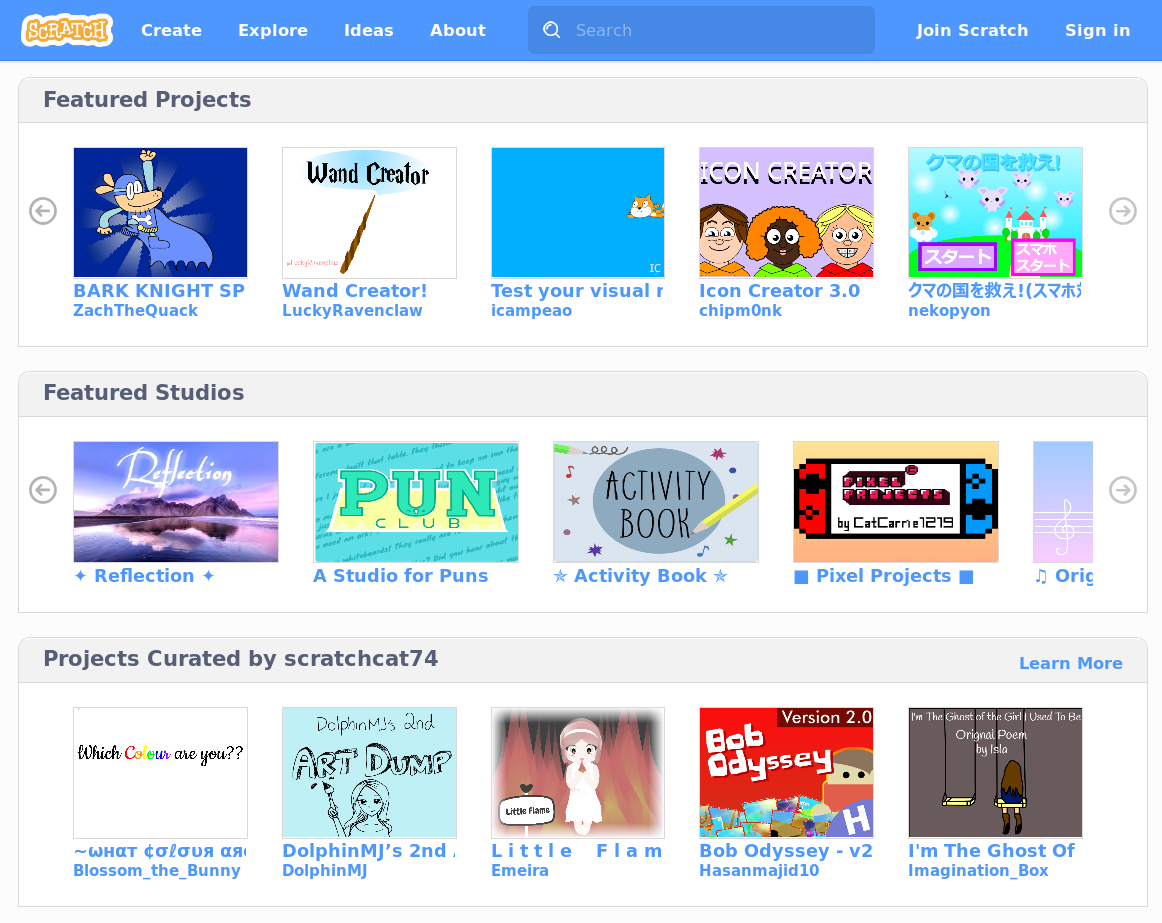
\includegraphics[width=.7\textwidth]{scratch-repository}
        \caption{Scratch's online repository}
    \end{figure}
\end{frame}

\begin{frame}[shrink=0]\frametitle{Why Scratch? Scratch's online community}
    % This repository encompasses over 38 million Scratch projects from over 36 million users at the time of writing
    % With over a million projects uploaded each month
    \begin{figure}
        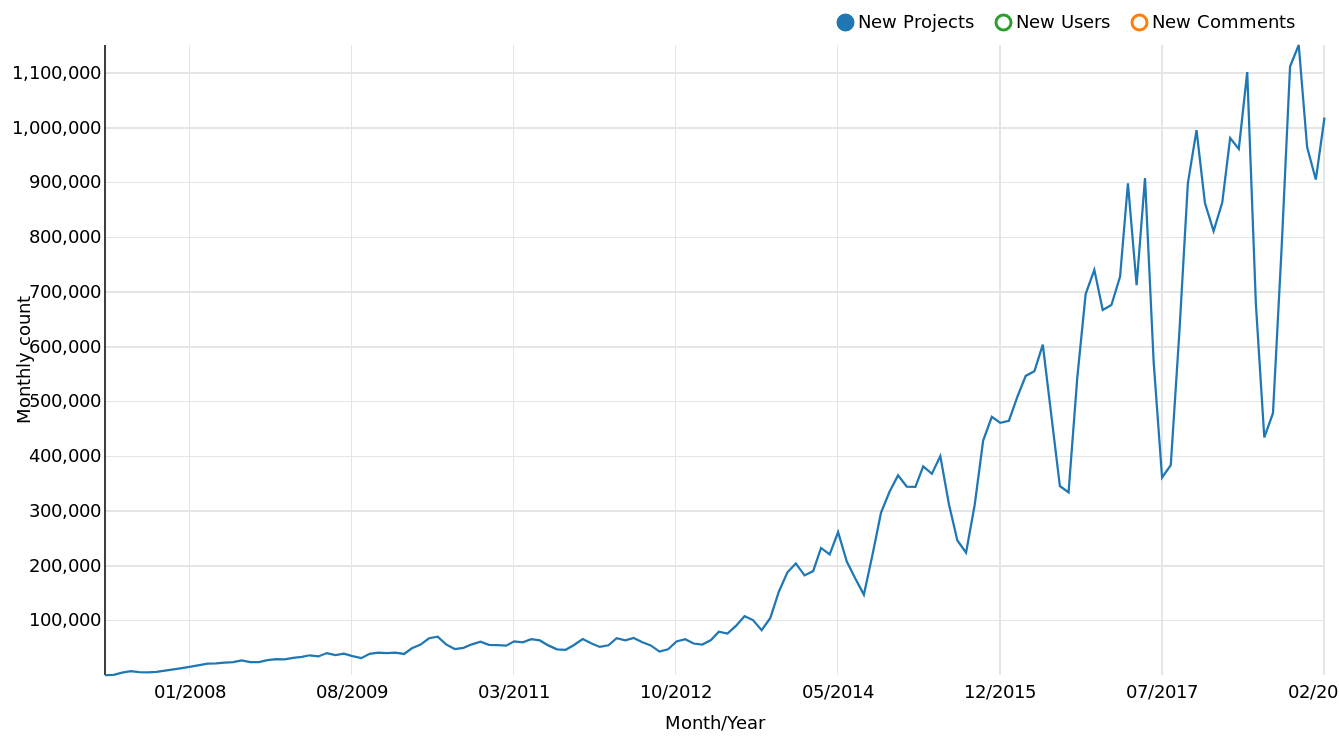
\includegraphics[width=.7\textwidth]{scratch-popularity}
        \caption{Submitted Scratch projects per month}
    \end{figure}
    \centering
    \begin{minipage}{.7\textwidth}
        \begin{itemize}
            \item over 38 million projects shared
            \item over 36 million users
        \end{itemize}
    \end{minipage}
\end{frame}

\begin{frame}\frametitle{Why Scratch? Good introduction to programming}
    % But more importantly Scratch is used by many schools and universities to introduce students to the principles of programming
    % Scratch is very suitable for this task for multiple reasons
    Many schools and universities deploy Scratch as a gentle introduction to programming
\end{frame}

\begin{frame}\frametitle{Why Scratch? Good introduction to programming}
    % For one thing, Scratch makes it impossible to write invalid code
    % The block-based code system eliminates the possibility of syntax errors
    % Blocks are chosen from a drawer
    % And even variable names can't be misspelled since they are chosen from a list
    % This all helps make Scratch very intuitive to use
    \centering
    Intuitive: Block based code system only allows valid code\\[\medskipamount]
    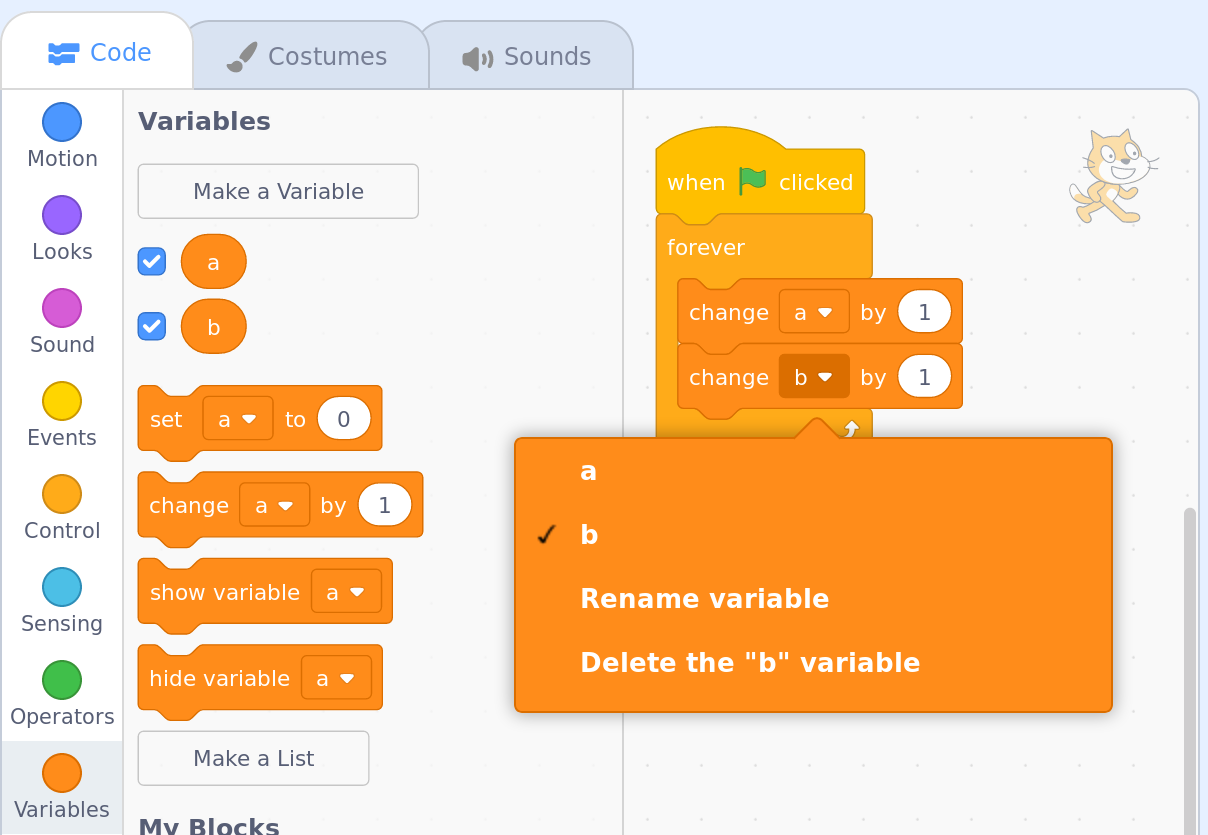
\includegraphics[width=.8\textwidth]{scratch-valid-code}
\end{frame}

\begin{frame}\frametitle{Why Scratch? Good introduction to programming}
    % At the same time, Scratch is very engaging
    % User input, graphics and audio are easy to integrate, which often leads to game-like programs
    \centering
    Engaging: User interaction, easy integration of graphics and sounds\\[\medskipamount]
    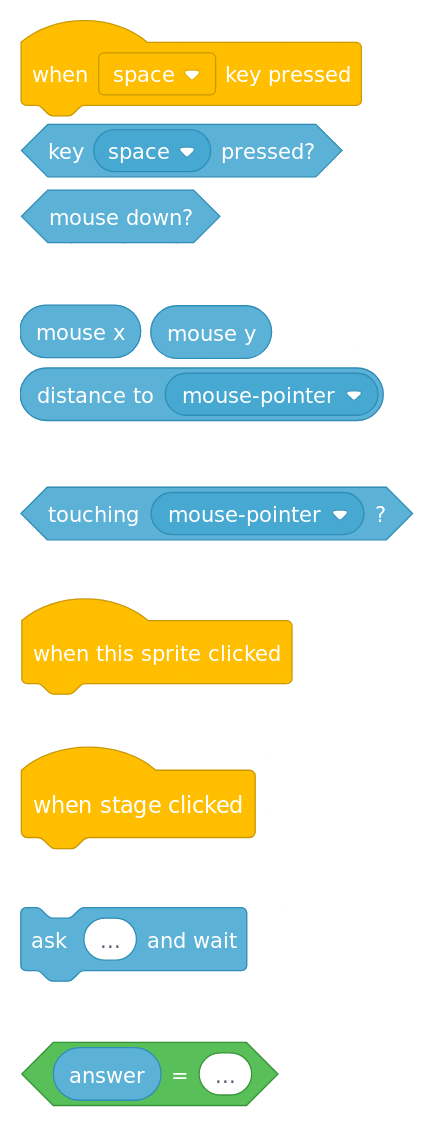
\includegraphics[width=.33\textwidth]{scratch-input-blocks}
    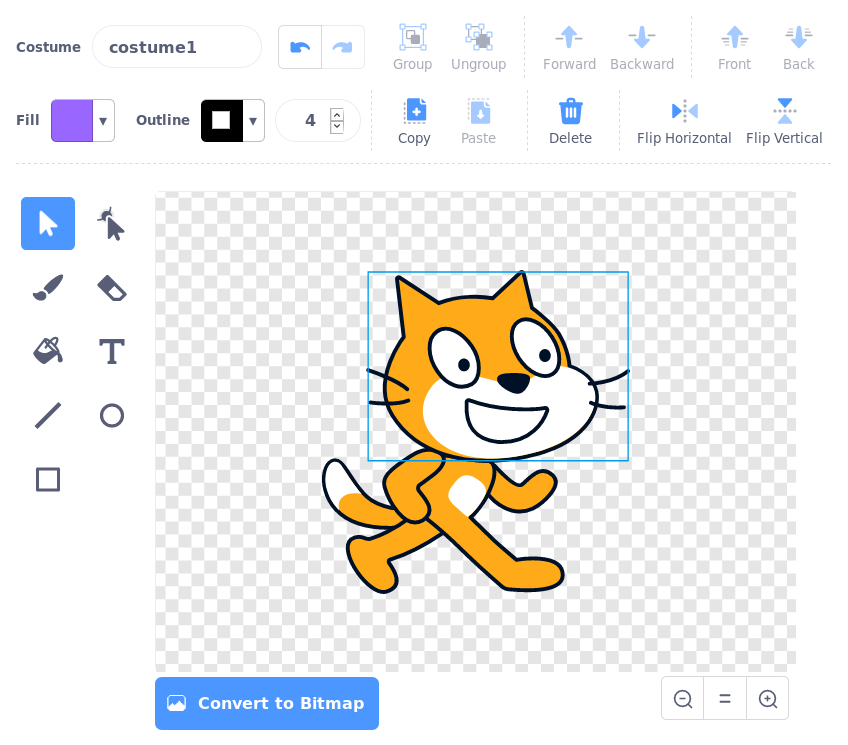
\includegraphics[width=.4\textwidth]{scratch-sprite-editor}
    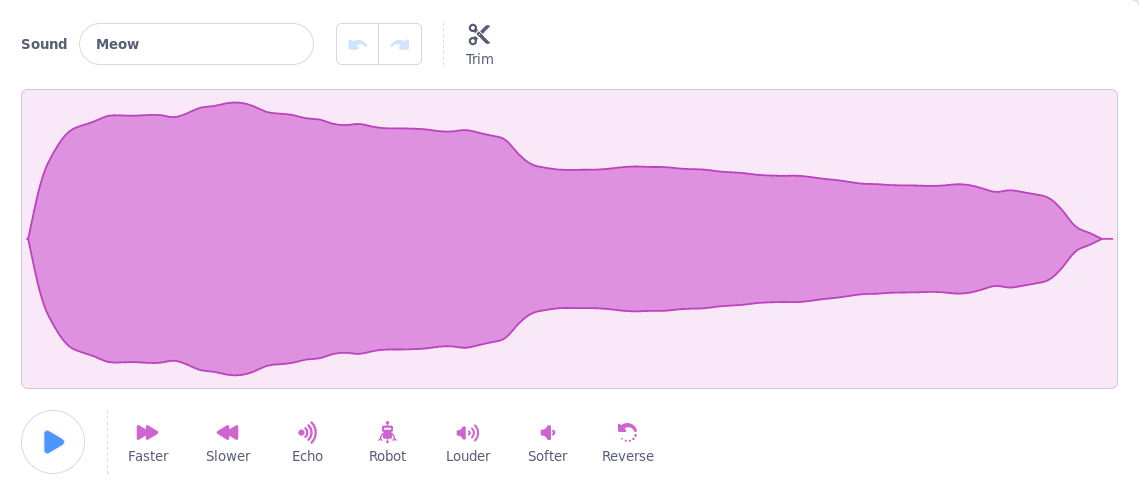
\includegraphics[width=.6\textwidth]{scratch-sound-editor}
\end{frame}

\begin{frame}
    \bigcenter{Why automated testing for Scratch?}
\end{frame}

\begin{frame}\frametitle{Why automated testing for Scratch?}
    Grading Scratch assignments is very time consuming
    \begin{itemize}
        \item every project has to be opened individually
        \item programs require large amounts of user interaction
    \end{itemize}

    \bigskip

    % TODO citation
    Some courses are attended by a large number of students ($> 200$), making manual grading infeasible.

    \bigskip

    Students can also use automated tests to get feedback for their own implementations.
\end{frame}

\begin{frame}
    \bigcenter{Why is automated testing for Scratch difficult?}
\end{frame}

\begin{frame}\frametitle{Why is automated testing for Scratch difficult?}
    Usually functional testing is deployed to automatically assess student solution,
    but this is not straightforward for Scratch
    \begin{itemize}
        \item Scratch is only accessible through its GUI
        \item no functions that take parameters and return a value
        \item no textual IO, keyboard and mouse input and graphical output
    \end{itemize}

    \bigskip

    \centering
    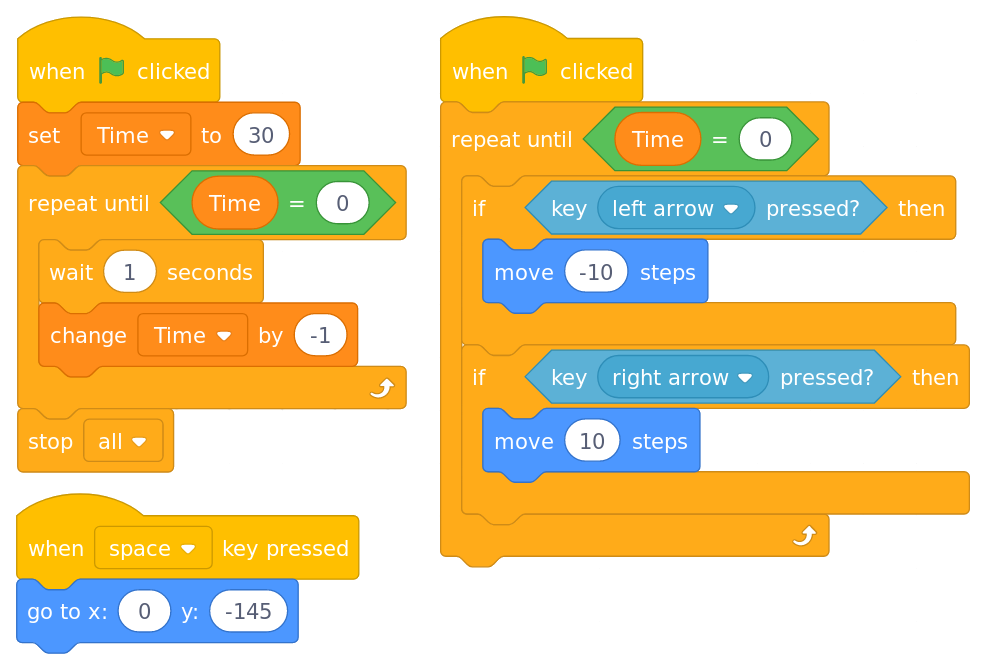
\includegraphics[width=.45\textwidth]{scratch-code}
    \hspace{1em}
    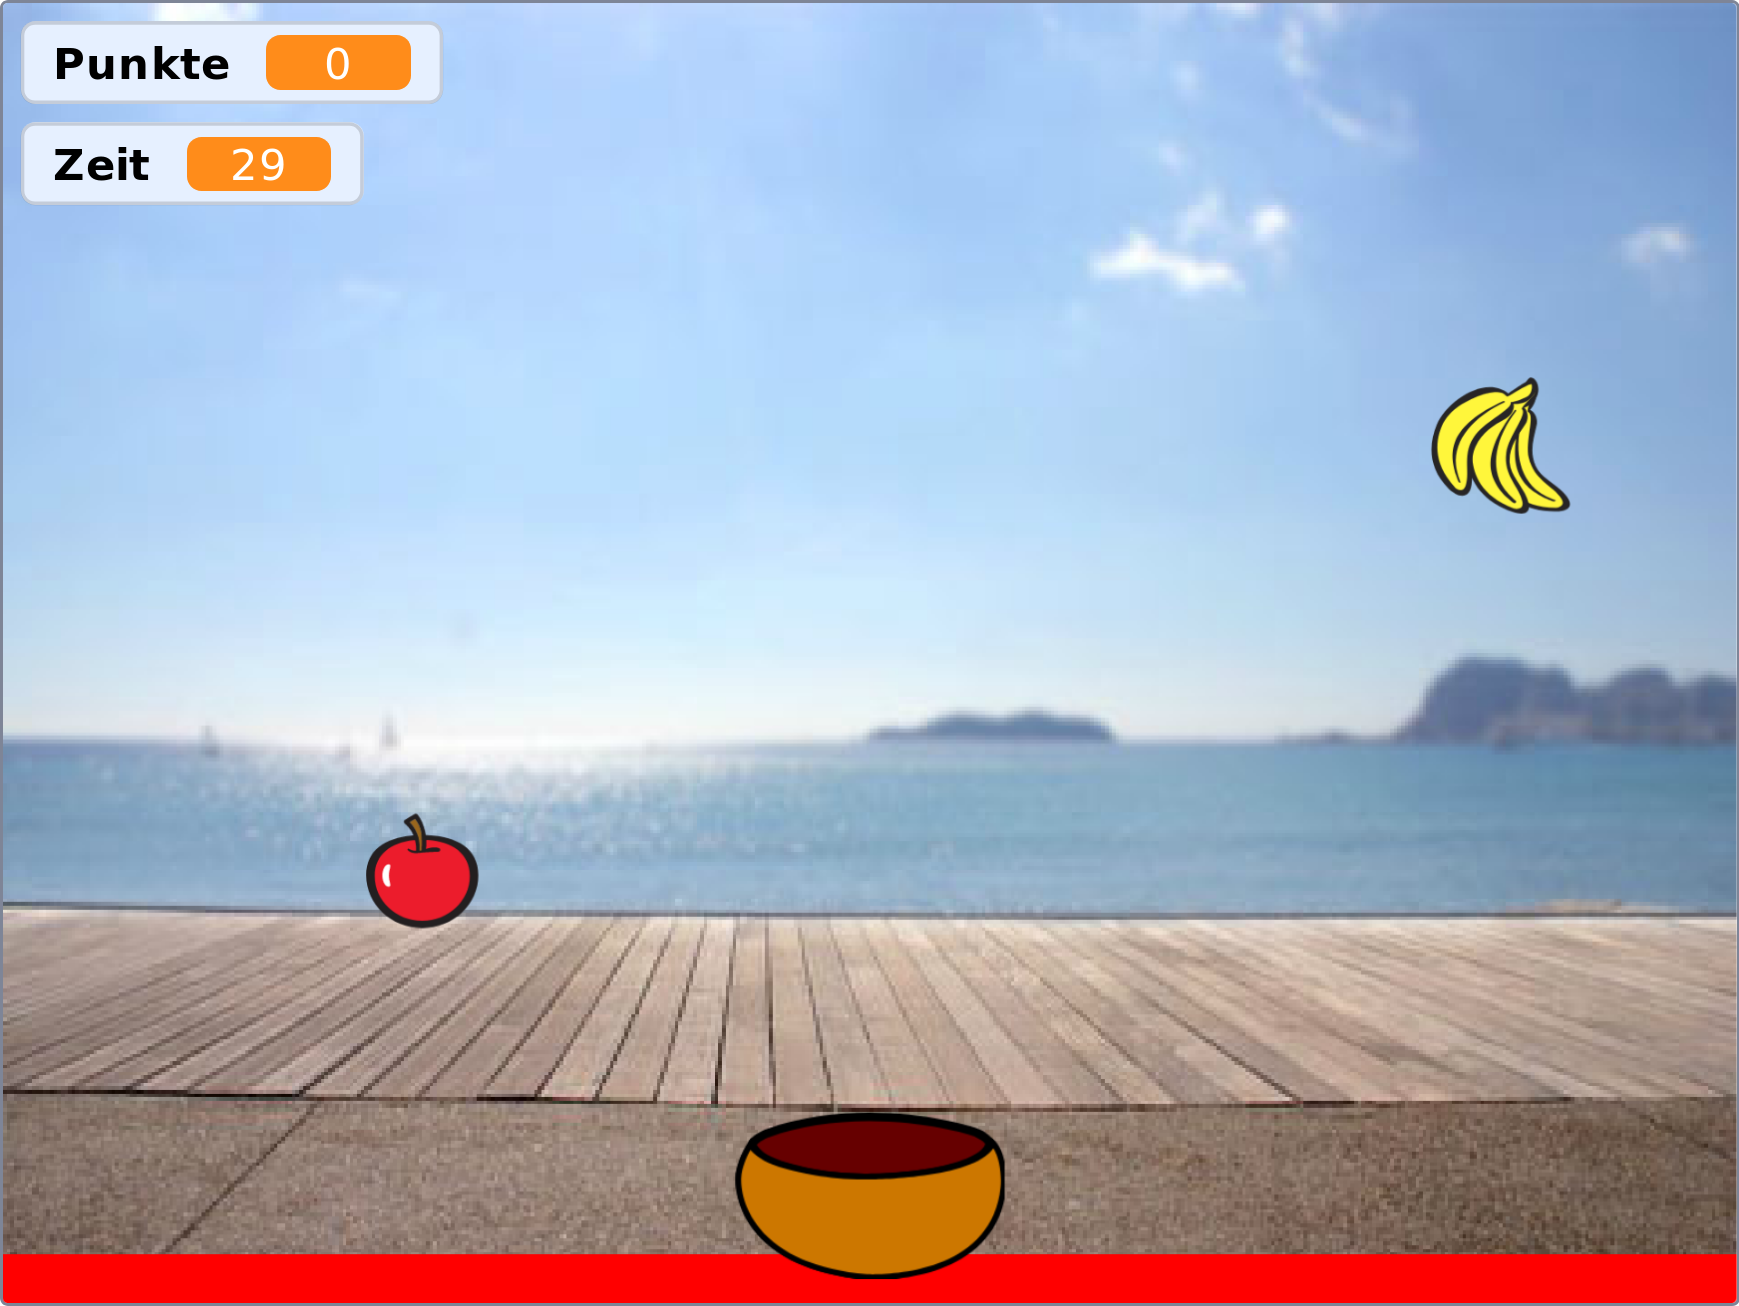
\includegraphics[width=.4\textwidth]{scratch-stage}
\end{frame}

\begin{frame}
    \bigcenter{How to automatically test Scratch programs?}
\end{frame}

\begin{frame}[fragile]\frametitle{How to automatically test Scratch programs?}
    Approach: Test on a system level by automating Scratch's IO

    \bigskip
    \centering

    \tikzset{>=latex,
           arrow/.style={draw, -{Latex[length=1.5mm, width=1.5mm]}},
             put/.style={draw, minimum height=0.65cm, minimum width=1.75cm, rounded corners, fill=red!20, text width=2.4cm, text centered},
              vm/.style={draw, minimum height=1.75cm, minimum width=3.0cm, rounded corners, fill=white},
             gui/.style={draw, minimum height=2.6cm, minimum width=3.5cm, rounded corners, fill=blue!20},
         whisker/.style={draw, minimum height=2.6cm, minimum width=3.5cm, rounded corners, fill=green!20},
             box/.style={draw,text centered, rounded corners}}

    \begin{tikzpicture}[scale=0.9, every node/.style={scale=0.9}]
        \node[box] at (0.0, 4.0) (input)  {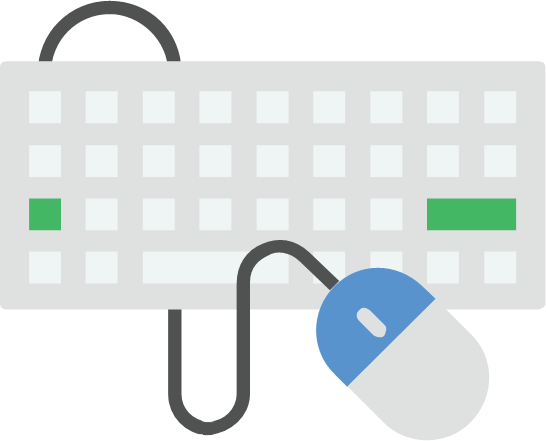
\includegraphics[height=.25\textheight]{mouse-keyboard}};
        \node[box] at (8.1, 4.0) (output) {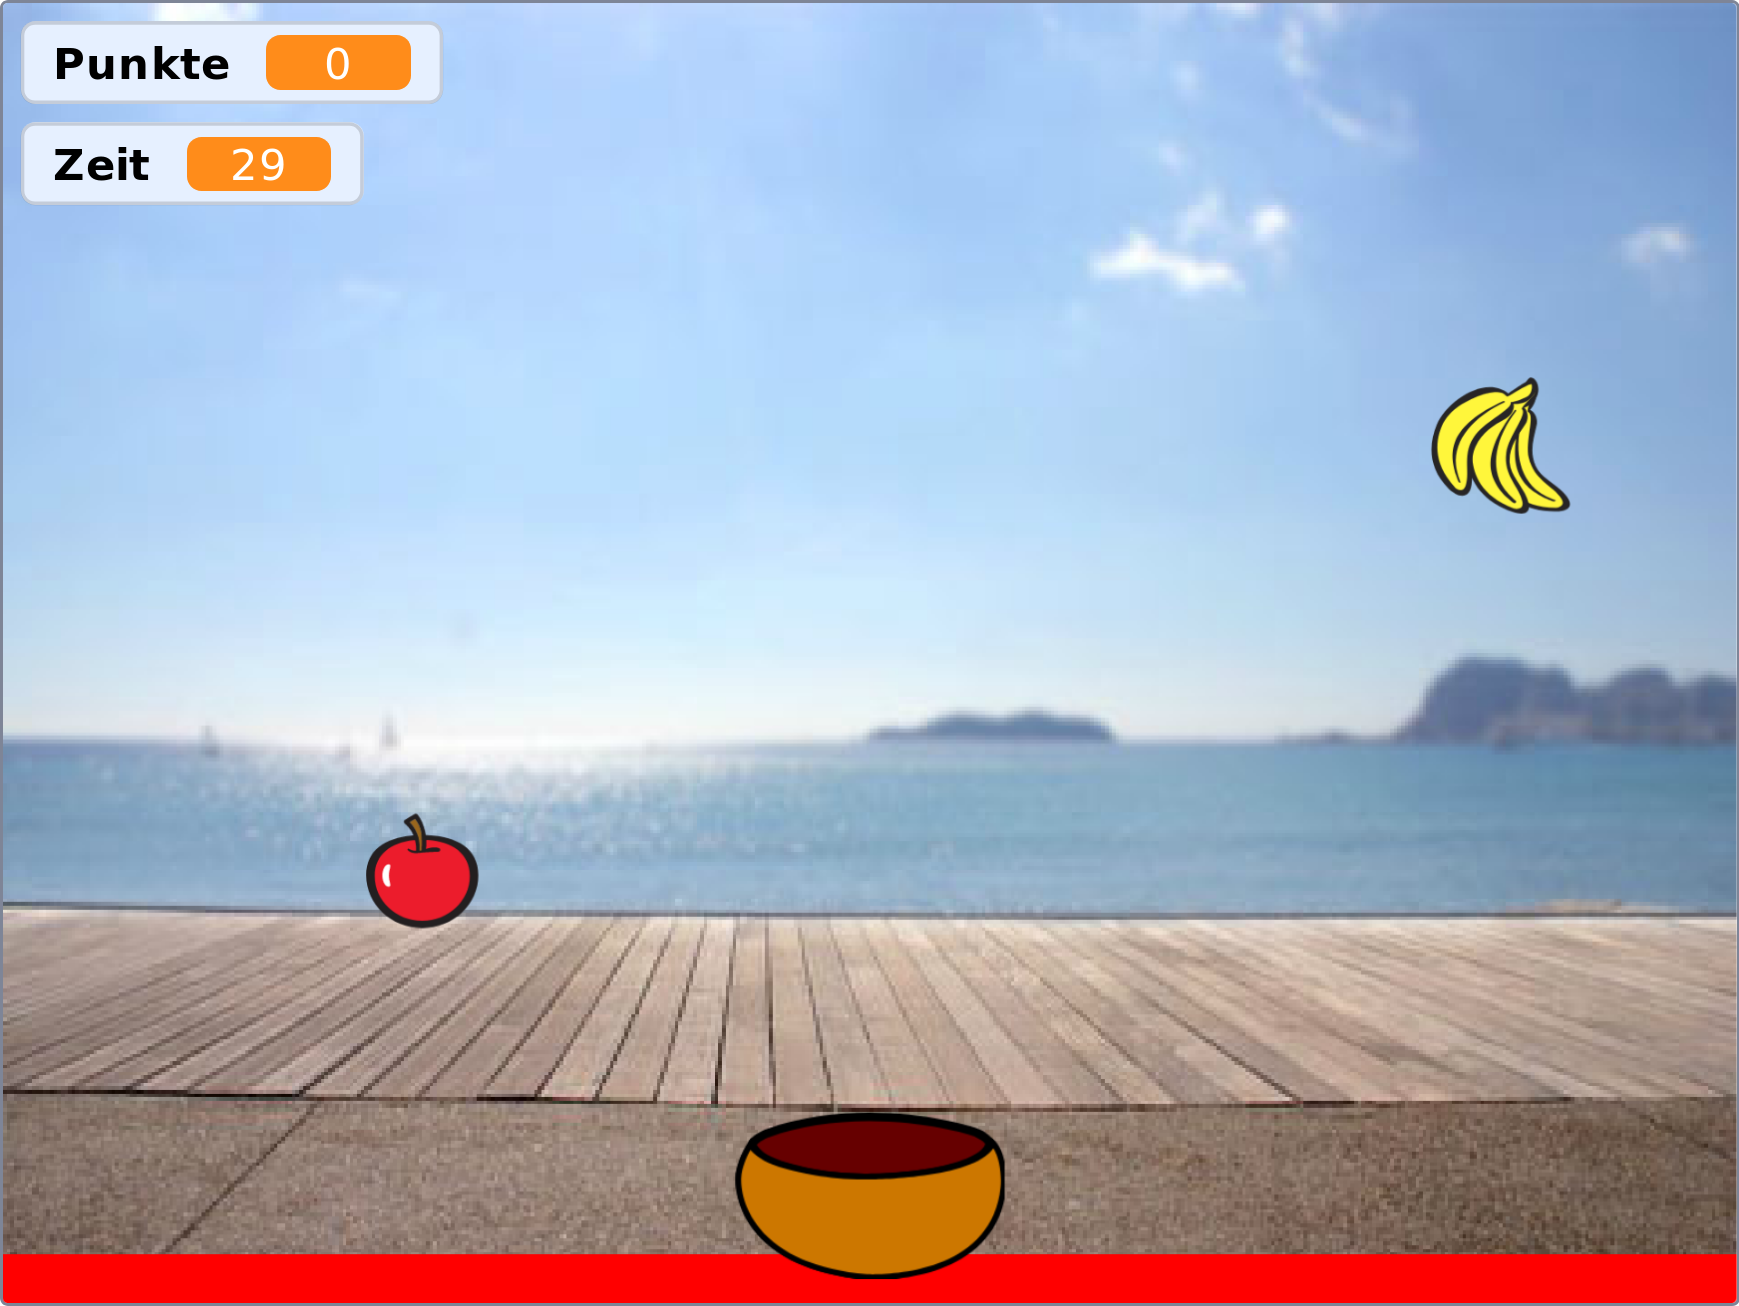
\includegraphics[height=.25\textheight]{scratch-stage}};

        \node[] at (0.0, 5.5) (inputtxt)  {\textbf{Input}};
        \node[] at (8.1, 5.5) (outputtxt) {\textbf{Output}};

        \begin{scope}[on background layer]
            \node[gui] at (4.0,  4.0)  (gui) {};
            \node[vm]  at (4.0,  3.75) (vm)  {};
        \end{scope}

        \node[put] at (4.0,  3.5) (put)     {\small Program under test};
        \node[]    at (4.0,  4.3) (vmtxt)   {\small Scratch VM};
        \node[]    at (4.0,  4.95) (guitxt) {\textbf{Scratch GUI}};

        \draw [shorten >= 2pt, shorten <= 2pt, arrow] (input) -- (gui);
        \draw [shorten >= 2pt, shorten <= 2pt, arrow] (gui)   -- (output);
    \end{tikzpicture}

    \bigskip

    \begin{tikzpicture}[scale=0.9, every node/.style={scale=0.9}]
        \node[box] at (-0.1, 4.0) (input) {
            \begin{minipage}{.28\textwidth}
                \begin{minted}[autogobble, breaklines, fontsize=\scriptsize, frame=none]{javascript}
                    t.inputImmediate({
                        device: 'mouse',
                        isDown: true,
                        x: 50,
                        y: 100
                    });
                \end{minted}
            \end{minipage}
        };

        \node[box] at (8.1, 4.0) (output) {
            \begin{minipage}{.28\textwidth}
                \begin{minted}[autogobble, breaklines, fontsize=\scriptsize, frame=none]{javascript}
                    sprite.x
                    sprite.y
                    sprite.rotation
                    sprite.sayText
                    sprite.costume
                    variable.value
                \end{minted}
            \end{minipage}
        };

        \node[] at (0.0, 5.5) (inputtxt)  {\textbf{Input}};
        \node[] at (8.1, 5.5) (outputtxt) {\textbf{Output}};

        \begin{scope}[on background layer]
            \node[whisker] at (4.0,  4.0)  (whisker) {};
            \node[vm]      at (4.0,  3.75) (vm)      {};
        \end{scope}

        \node[put] at (4.0,  3.5)  (put)        {\small Program under test};
        \node[]    at (4.0,  4.3)  (vmtxt)      {\small Scratch VM};
        \node[]    at (4.0,  4.95) (whiskertxt) {\textbf{Whisker}};

        \draw [shorten >= 2pt, shorten <= 2pt, arrow] (input)   -- (whisker);
        \draw [shorten >= 2pt, shorten <= 2pt, arrow] (whisker) -- (output);
    \end{tikzpicture}

    % \begin{figure}
    %     \centering
    %     \tikzset{>=latex,
    %            arrow/.style={draw, -{Latex[length=1.5mm, width=1.5mm]}},
    %              put/.style={draw, minimum height=1.7cm, minimum width=3.5cm, rounded corners, fill=red!20, text width=2.5cm, text centered},
    %               vm/.style={draw, minimum height=3.0cm, minimum width=6.0cm, rounded corners, fill=white},
    %              gui/.style={draw, minimum height=4.2cm, minimum width=7.0cm, rounded corners, fill=blue!20},
    %              box/.style={draw, minimum height=4.2cm, minimum width=4.0cm, rounded corners, text width=3.5cm},
    %           boxtxt/.style={minimum width=4.0cm, rounded corners, text width=3.5cm}}

    %      \begin{tikzpicture}[scale=0.6, every node/.style={scale=0.6}]
    %         \begin{scope}[on background layer]
    %             \node[gui] at (0.0,  0.4) (gui)     {};
    %             \node[vm]  at (0.0,  0.0) (vm)      {};
    %         \end{scope}

    %         \node[put]     at (0.0, -0.4) (put)     {\Large \textbf{Program under test}};
    %         \node[]        at (0.0,  1.0) (vmtxt)   {\Large \textbf{Scratch Virtual Machine}};
    %         \node[]        at (0.0,  2.0) (guitxt)  {\Large \textbf{Scratch GUI}};
    %         \node[box, left=of gui]       (input)   {};
    %         \node[box, right=of gui]      (output)  {};
    %         \node[boxtxt, below right] at ([yshift=-2mm] input.north west)  (inputtxt)
    %             {\centering {\LARGE \textbf{Input}}\\[.5\baselineskip]\LARGE Key presses, mouse movement, mouse clicks, etc.};
    %         \node[boxtxt, below right] at ([yshift=-2mm] output.north west) (outputtxt)
    %             {\centering {\LARGE \textbf{Output}}\\[.5\baselineskip]\LARGE Visual animations, audio, etc.};

    %         \path [arrow] (input) -- (gui);
    %         \path [arrow] (gui)   -- (output);
    %     \end{tikzpicture}
    %     \caption{Input and output of the Scratch GUI}
    % \end{figure}


\end{frame}
